\providecommand{\main}{../../..}
\documentclass[\main/dresen_thesis.tex]{subfiles}
  \renewcommand{\thisPath}{\main/chapters/monolayers/magneticStructure}

\begin{document}

  \subsection{Magnetism of Square Array Monolayers}
  \begin{figure}[tb]
    \centering
    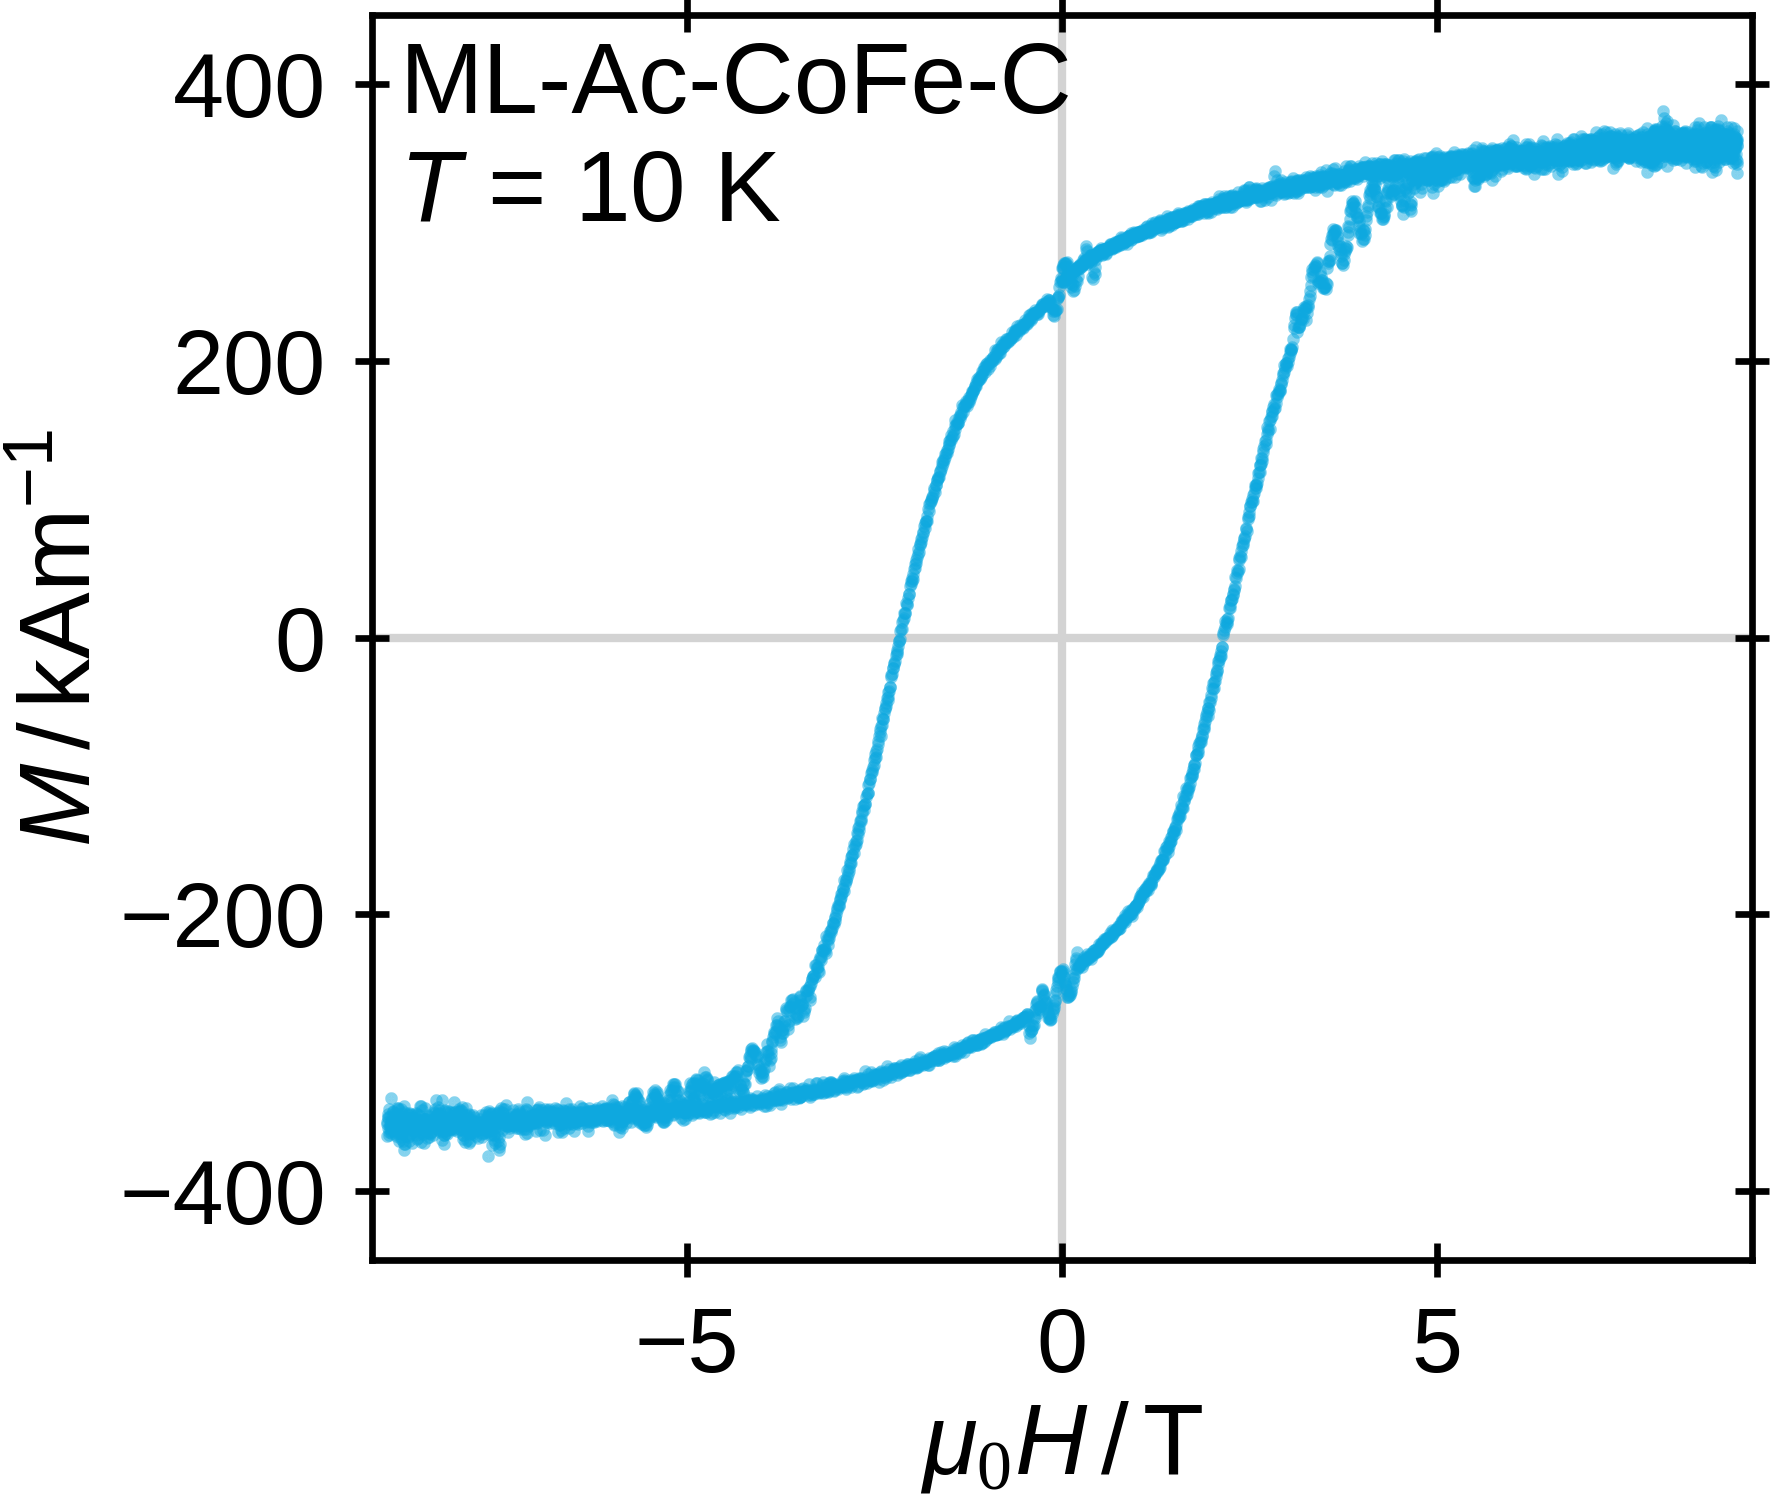
\includegraphics{monolayer_PPMS_VSM_10K_ML_Ac_CoFe_C}
    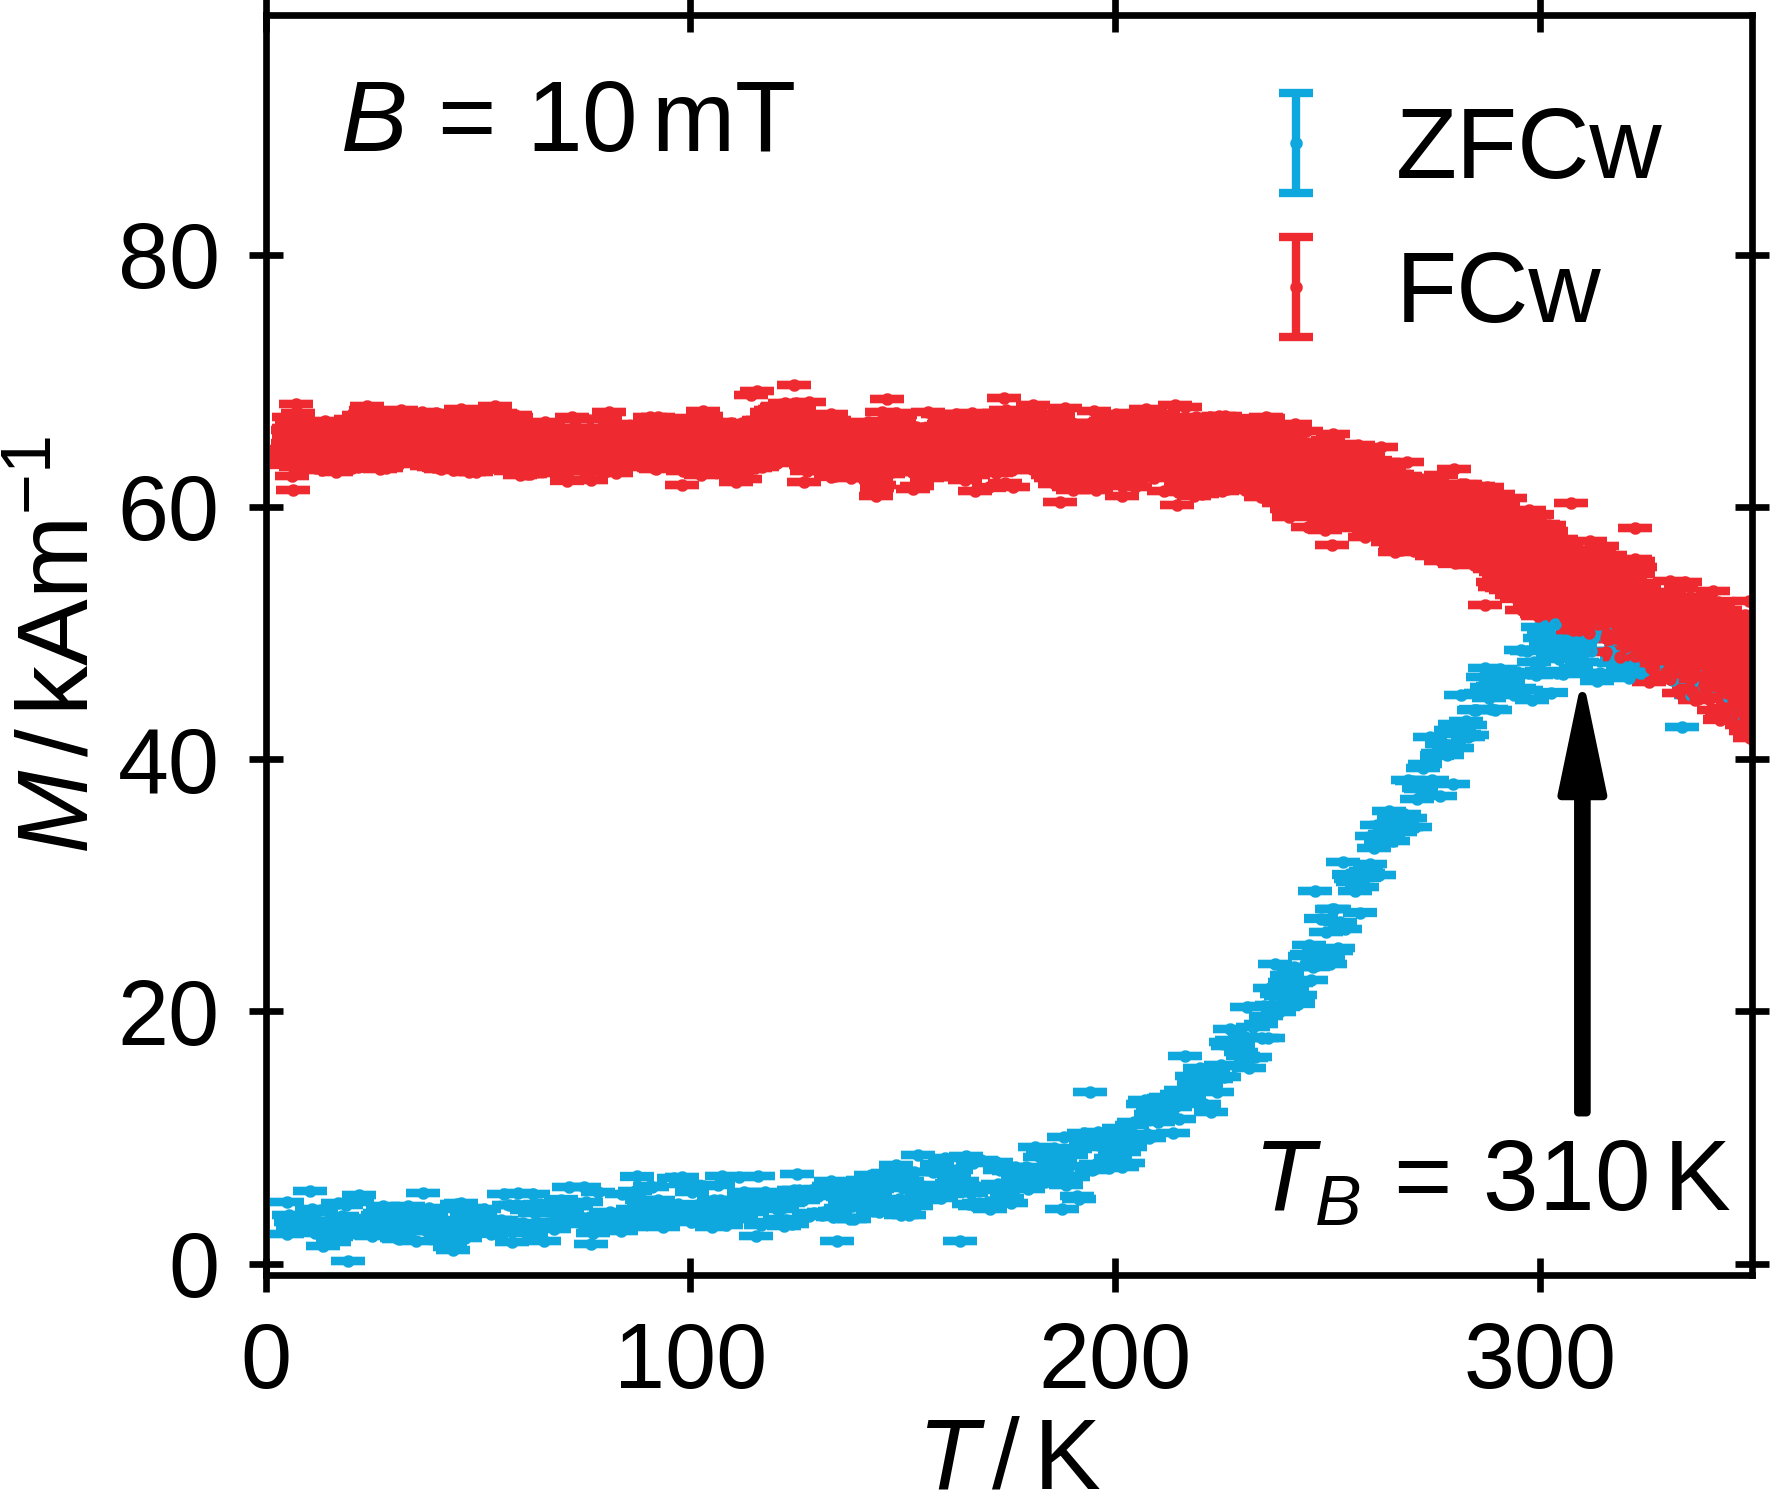
\includegraphics{monolayer_PPMS_ZFC_FC_ML_Ac_CoFe_C}
    \caption{\label{fig:monolayer:magneticStructure:ppms}Low temperature hysteresis (left) and temperature dependent magnetization (right) of ordered monolayer prepared from Ac-CoFe-C.}
  \end{figure}
  After drop-casting cubic nanoparticles in a ordered square lattice, the measured low-temperature hysteresis loop changes drastically from the behaviour observed for the unordered case obtained from measuring a frozen dispersion.
  As can be seen in \reffig{fig:monolayer:magneticStructure:ppms} (left), the hysteresis loop shows a strong jump around zero field, which is not visible in the measurement of the same nanoparticles that were frozen in dispersion in \reffig{fig:monolayers:nanoparticle:vsm10K} (right).
  The effect is visible up to a temperature of $150 \unit{K}$ as can be seen in \reffig{fig:monolayers:fig:monolayer:magneticStructure:ppmsTempDependent}.
  \begin{figure}[tb]
    \centering
    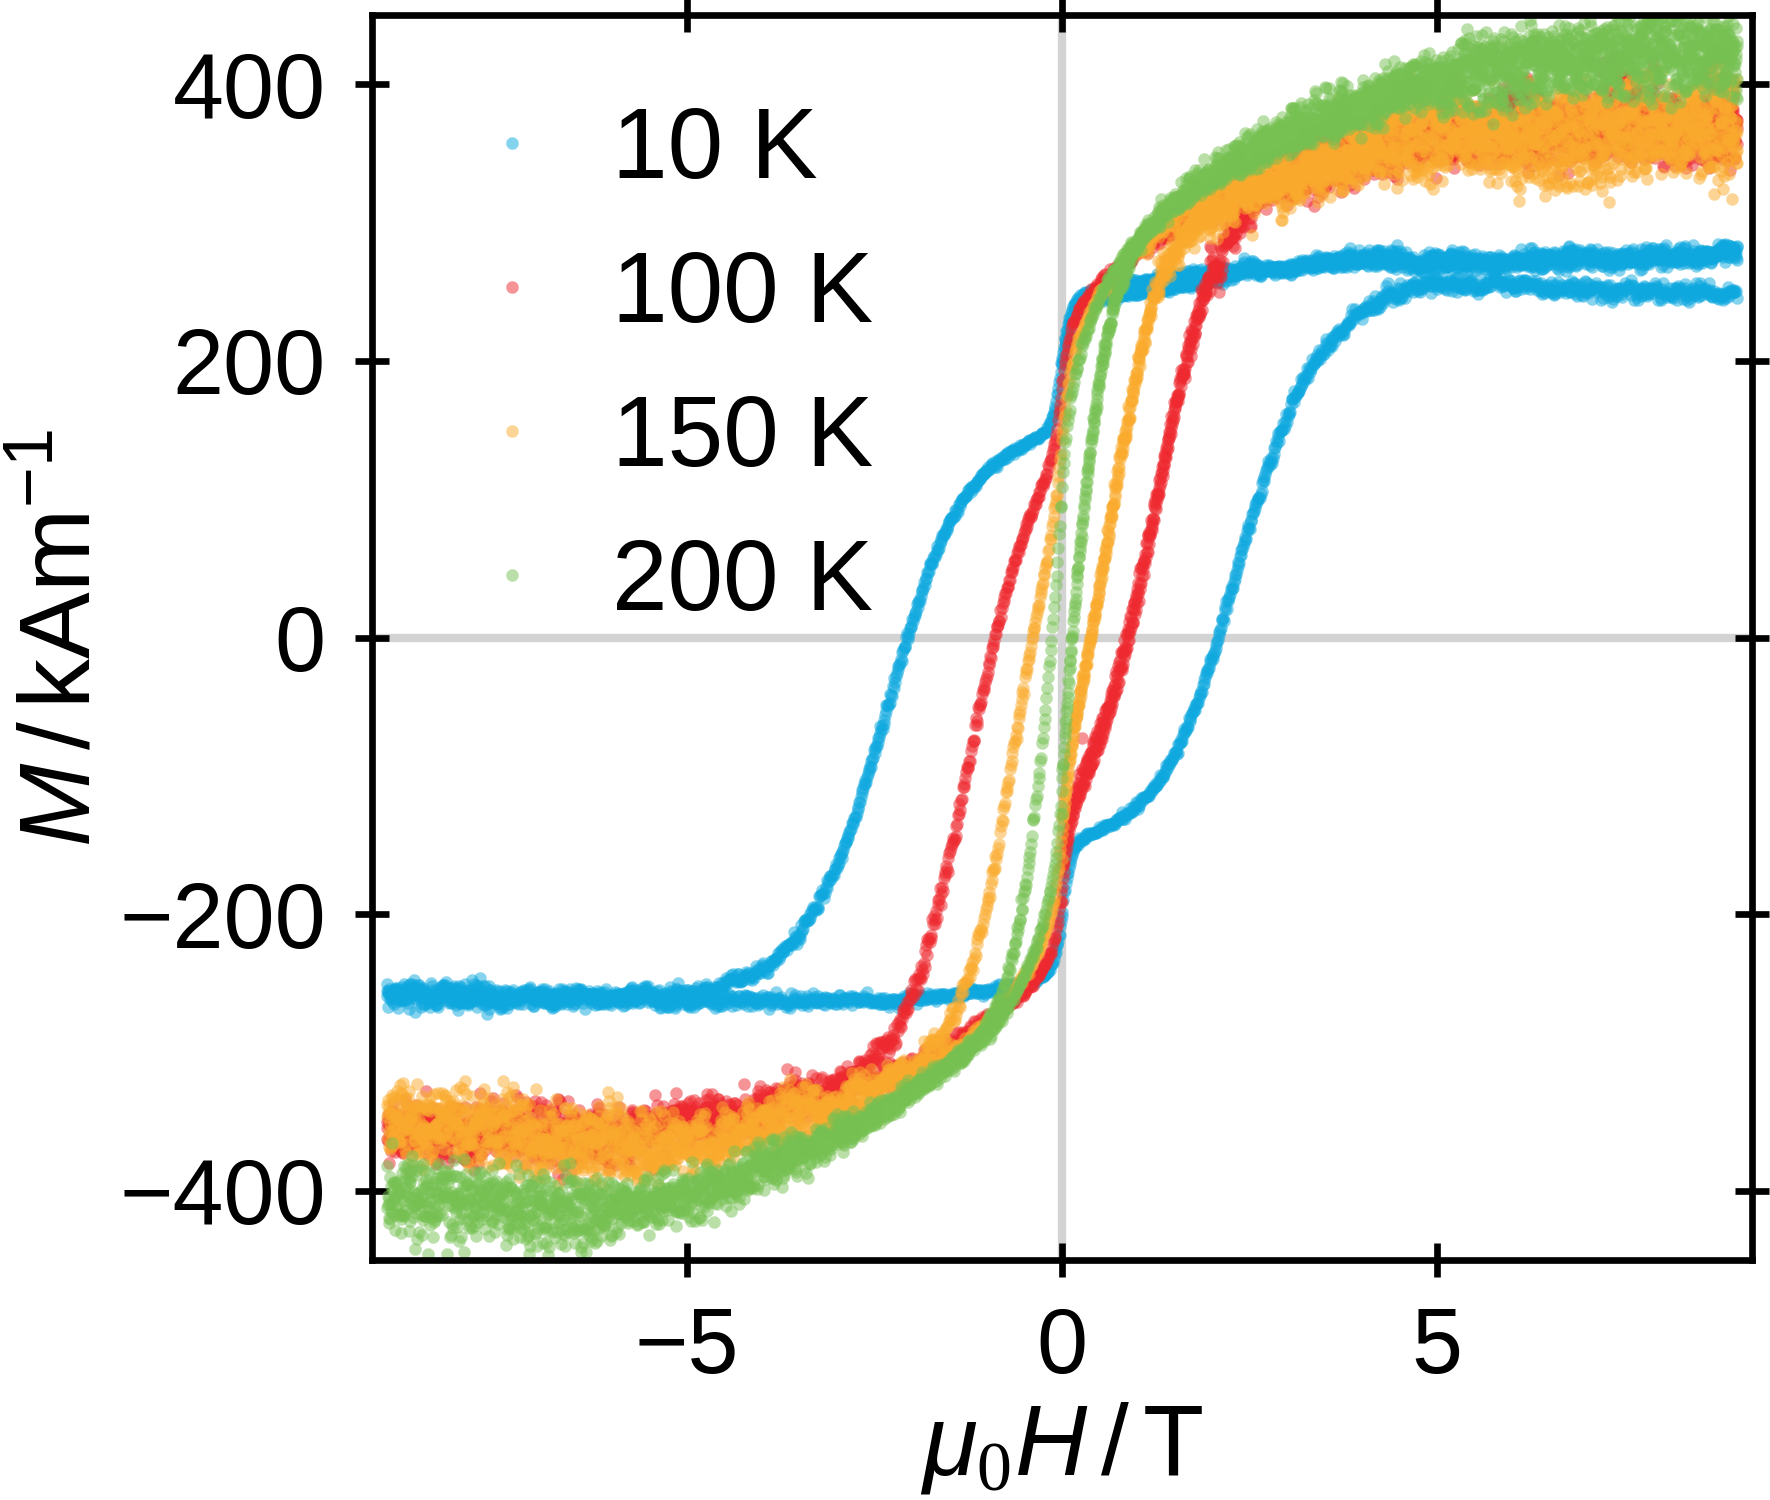
\includegraphics{monolayer_PPMS_VSM_multiTemps_ML_Ac_CoFe_C}
    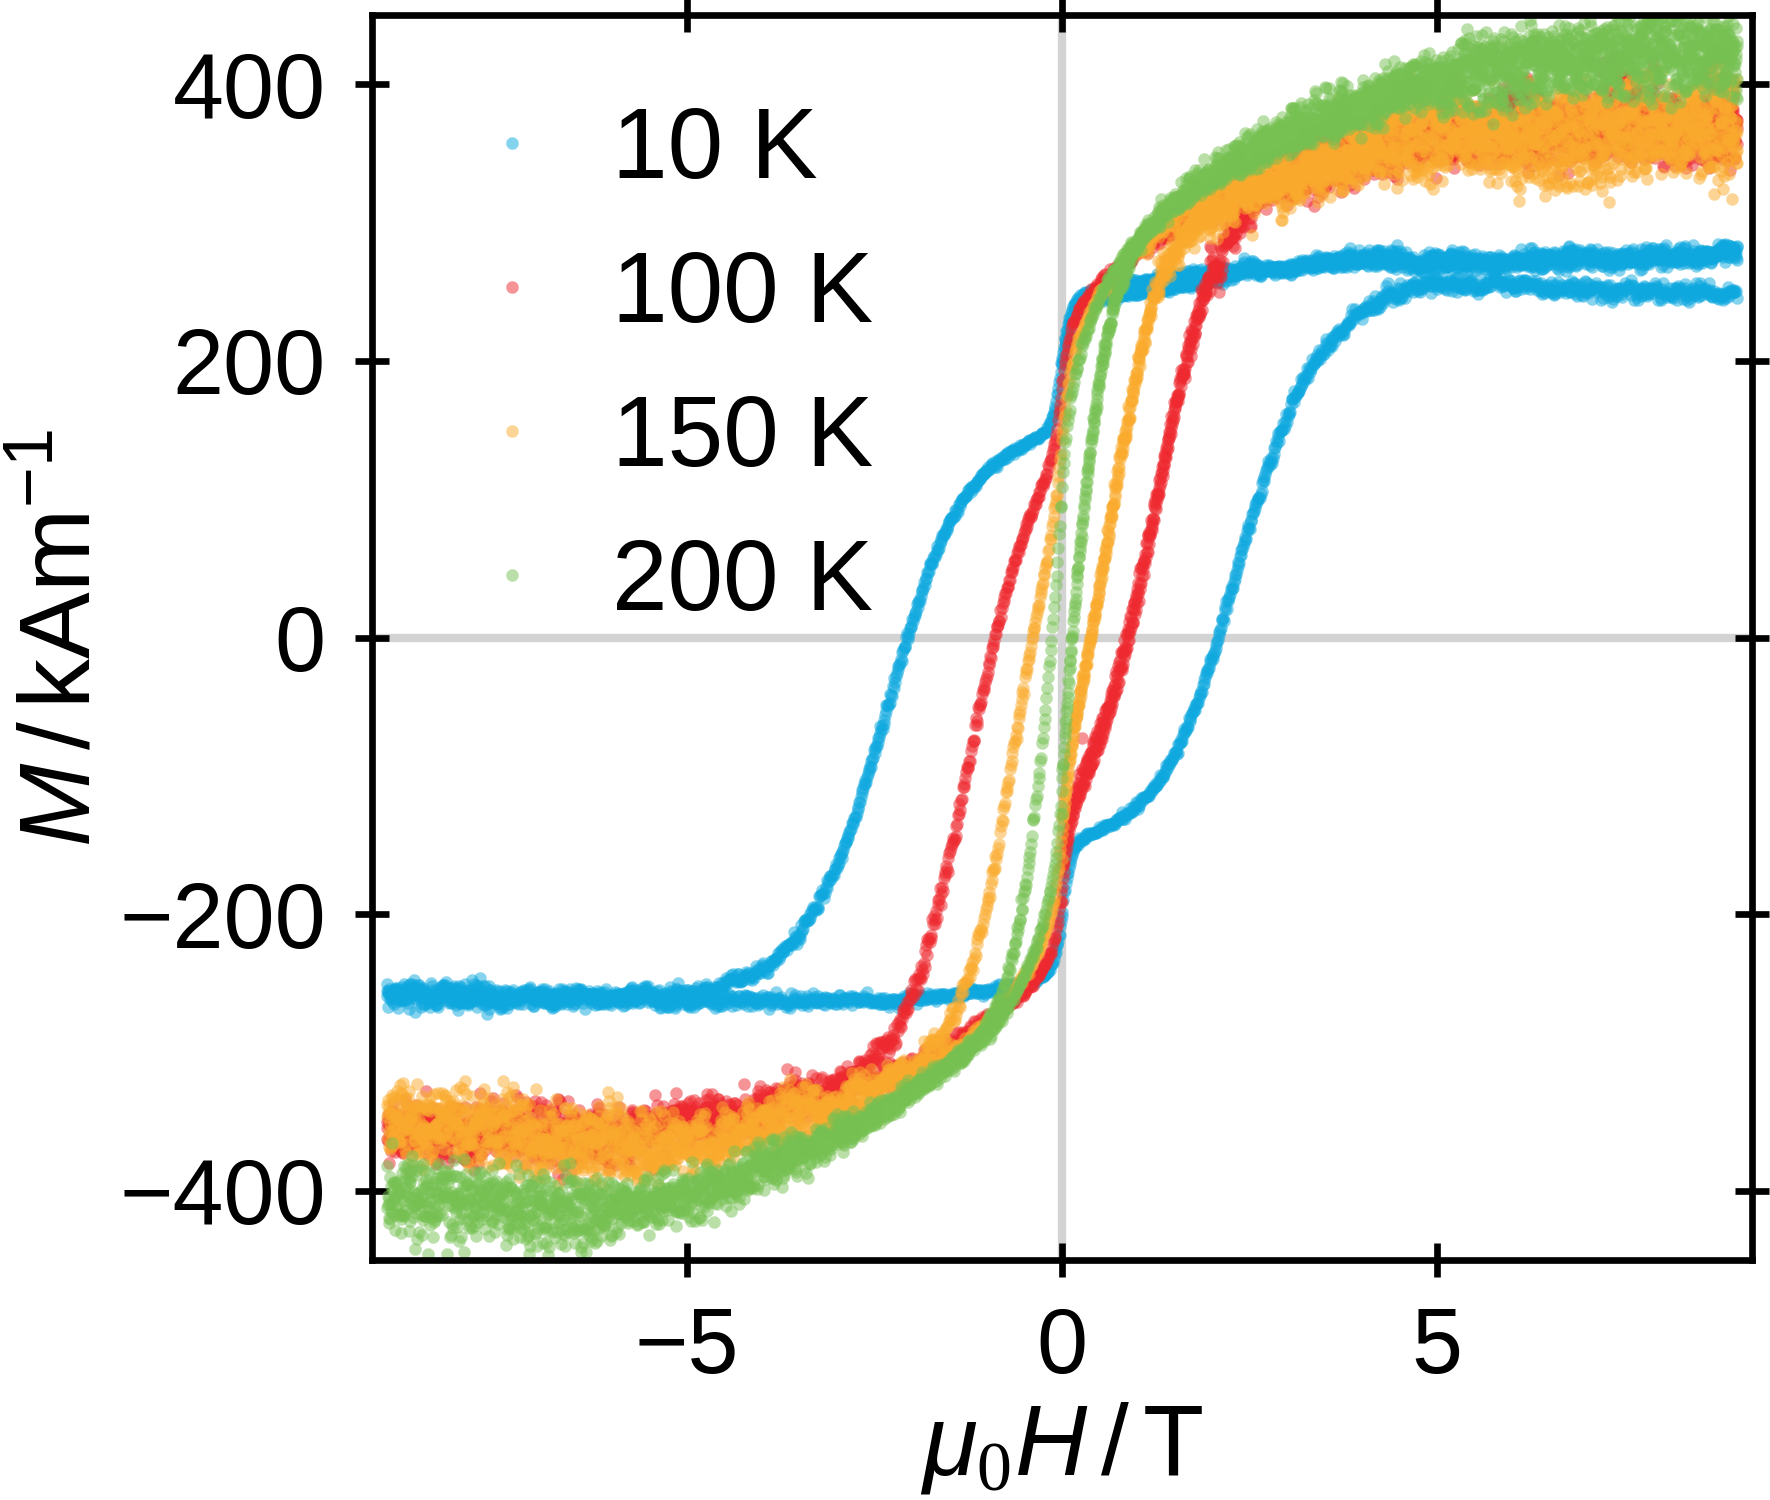
\includegraphics{monolayer_PPMS_VSM_multiTemps_ML_Ac_CoFe_C}
    \caption{\label{fig:monolayer:magneticStructure:ppms}Magnetic hysteresis measured at multiple temperatures (left).}
  \end{figure}
  
  % To understand whether effects of magnetic interparticle interactions emerge from the structure, the expected magnetic structure of long range ordered nanoparticles in the plane is discussed in the following and selected sample characterizations via vibrating sample magnetometry (VSM) and polarized grazing incidence small angle neutron scattering (polGISANS) are presented.
  % The results are compared to the single particle properties obtained from the nanoparticle in dispersion, as well as to the theory to deduce upon emergent properties.


  %   \subfile{\thisPath/theory/theory}
  %   \FloatBarrier

  % \subsection{Magnetic Characterization of a Cobalt Ferrite Monolayer}
  %   Yo
  %   \FloatBarrier

  % \subsection{Discussion}
  %   Yo
  %   \FloatBarrier
\end{document}